\NeedRoom{10}

\subsection{Fleet Sensitivity}

\begin{figure}[htbp]\centering

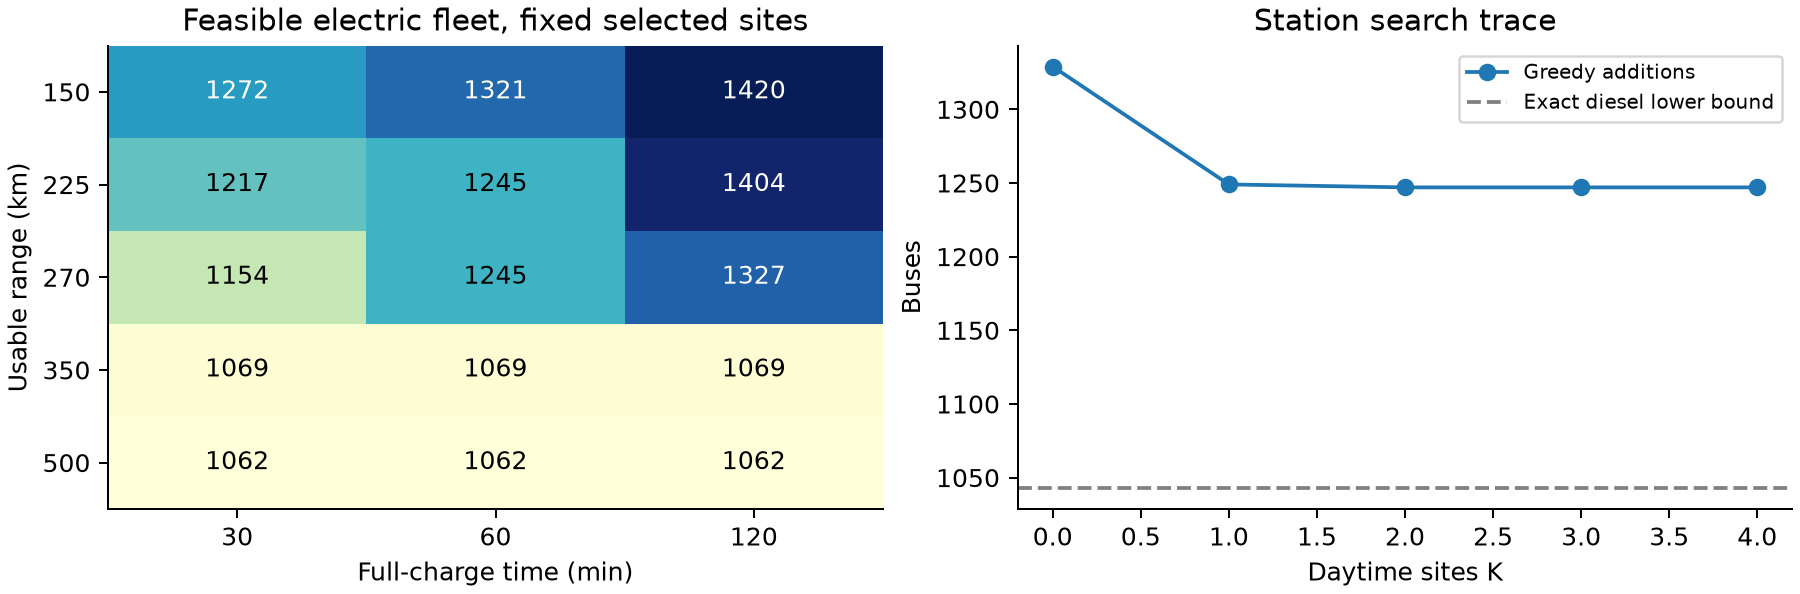
\includegraphics[width=\textwidth,height=0.37\textheight,keepaspectratio]{images/fleet_sensitivity.png}

\caption{Validated fleet upper bounds at fixed selected sites, and the greedy station-addition trace.}\label{fig:result1}

\end{figure}

The true optimum cannot increase when R increases or T decreases. The heuristic can miss that property because different block partitions hide different opportunities. We retain and validate earlier feasible incumbents under relaxed parameters. Both raw and retained counts are recorded.


The station curve shows the greedy addition path. Subsequent exchanges may change the final set. A plateau is specific to the tested candidates and partitions, not proof that further infrastructure is useless. A separate cost screen minimizes bus list price plus a fixed site allowance over the delivered trace; it excludes charger power, grid connection, land and maintenance, and does not solve the mixed-cost location model globally.


Its minimum-cost trace points have K = 2 for Vancouver, 1 for Chicago and 3 for London. These are screening outcomes over the same candidate traces, not certified station counts.


\begin{longtable}{@{}L{\dimexpr 0.30000\textwidth-2\tabcolsep\relax}L{\dimexpr 0.22000\textwidth-2\tabcolsep\relax}L{\dimexpr 0.48000\textwidth-2\tabcolsep\relax}@{}}
\caption{Fleet response to alternate distance assumptions}\label{tab:source7}\\
\toprule
\textbf{Additional check} & \textbf{Electric buses} & \textbf{Interpretation} \\
\midrule
\endfirsthead
\multicolumn{3}{l}{Table \thetable\ (continued)}\\
\toprule
\textbf{Additional check} & \textbf{Electric buses} & \textbf{Interpretation} \\
\midrule
\endhead
\midrule\multicolumn{3}{r}{Continued on next page}\\\endfoot
\bottomrule\endlastfoot
distance\_lower & 1188 & Independent assumption rerun \\
road\_stress & 1291 & Independent assumption rerun \\
\end{longtable}

Infinite range is solved by exact diesel matching. A production fleet would also require reserve vehicles, reliability margin, compatible body types and cross-day closure. Neither the active fleet nor its ratio to $N_d$ can be compared directly with inventory statistics containing maintenance and spare buses.

